\chapter{Techniky a princípy a ciele útokov}

\label{kap:teoria} % id kapitoly pre prikaz ref

V tejto kapitole stručne zhrnieme najčastejšie techniky používané na indukovanie chýb na hardvéri a vysvetlíme princípy týchto techník.

Základným predpokladom úspešného útoku pomocou indukovania chýb je fyzický prístup k zariadeniu, ktoré je cieľom útoku. Väčšina takýchto útokov vyžaduje miernu modifikáciu hardvéru, aby bolo možné ovplyvniť jeho činnosť, napríklad odstránenie niektorých komponentov, ktoré by mohli útok sťažiť, prípadne úplne znemožniť. Ideálnou možnosťou pre útočníka je, ak môže komponent vybrať a prevádzkovať ho vo svojom prostredí. V niektorých prípadoch sa dokonca podarilo zariadenie poškodiť na trvalo tak, aby chyba spôsobovala cielený účinok v systéme, do ktorého bolo následne opäť nasadené. Častými obeťami takýchto útokov sú vnorené (angl. embedded) zariadenia, väčšinou ovládané pomocou MCU (Micro Controller Unit), známe aj pod názvom mikrokontrolér. Práve pri vnorených zariadeniach sú zvyčajne splnené všetky vyššie uvedené predpoklady. 

\section{Zmena napätia}
Jednou z najjednoduchších a veľmi často využívaných techník indukovania chýb je zmena napätia, obvykle podpätie (angl. power glitch). Princíp takéhoto útoku spočíva v skonštruovaní obvodu, ktorý bude mať kontrolu nad napájaním zariadenia, na ktoré chceme útočiť a vo vhodných časových intervaloch veľmi krátkej dĺžky (rádovo stovky nanosekúnd), vyvolať prudkú zmenu napätia. Takáto manipulácia môže spôsobiť nedefinované správanie na napájanom zariadení, najčastejšie možno očakávať, že ovplyvní aktívne časti hardvéru, napríklad obvody na procesore vykonávajúce jednotlivé inštrukcie. Častými symptómami takéhoto útoku sú napríklad preskočenie inštrukcie, nekorektné vyhodnotenie podmieneného skoku, chybný výsledok aritmetickej, či logickej operácie a pod. Najdôležitejšia časť takéhoto útoku je správne načasovanie a dĺžka intervalu zmeny napätia. Pokiaľ je tento časový úsek zmeny napätia príliš dlhý (viac ako 2-3 mikrosekundy), je veľká pravdepodobnosť, že nastane fatálne zlyhanie a následný reštart zariadenia. Práve požadovaná presnosť časovania je parameter, ktorý výrazne vplýva na technickú náročnosť útoku. V niektorých prípadoch 

Pre implementáciu útoku využívajúceho techniku zmeny napätia sú zvyčajne potrebné dve základné súčasti. Jednou je obvod, ktorý dokáže dynamicky manipulovať s napájaním zariadenia, na ktoré cielime a druhým je generátor riadiacich impulzov pre tento obvod, ktorý dokáže generovať signály s dostatočnou presnosťou. V závislosti od zložitosti a požadovaných parametrov týchto dvoch komponentov sa odvíjajú aj náklady a náročnosť takéhoto útoku. V porovnaní s inými technikami však zmena napätia patrí k menej náročným na implementáciu a je preto veľmi často používaná. 

Príklad jednoduchej implementácie takéhoto útoku môže byť napríklad použitie tranzistora, ktorým vieme spínať napájanie na mikrokontroléri. Takýmto spôsobom vieme na krátky okamih vypnutím tranzistora vyvolať podpätie na mikrokontroléri a následným zopnutím zase vrátiť napätie do bežného stavu, čo môže vyvolať chybné vykonanie jednej alebo viacerých nasledujúcich inštrukcií \cite{vccOnTheCheap}.

Útok založený na podobnom, ale mierne zložitejšom princípe využíva tzv. \uv{Corwbars} obvod. Princíp takéhoto obvodu spočíva v tom, že okrem hardvéru, zdroj napájania paralelne zapojíme cez tranzistor do \uv{skratu}, ktorý vieme spínať pomocou tohoto tranzistora. Generovaním impulzov do tranzistora vieme na veľmi krátky čas vyskratovať napájací zdroj, čím spôsobíme prudké zmeny v napätí na mikrokontroléri. Aby bolo možné presnejšie zacieliť na konkrétnu časť vykonávaného kódu bolo ovládanie tohoto obvodu synchronizované s externými hodinami cieľového zariadenia, znázornené na obrázku \ref{obr:vccSync} \cite{crowbars}.

\begin{figure}
    \centerline{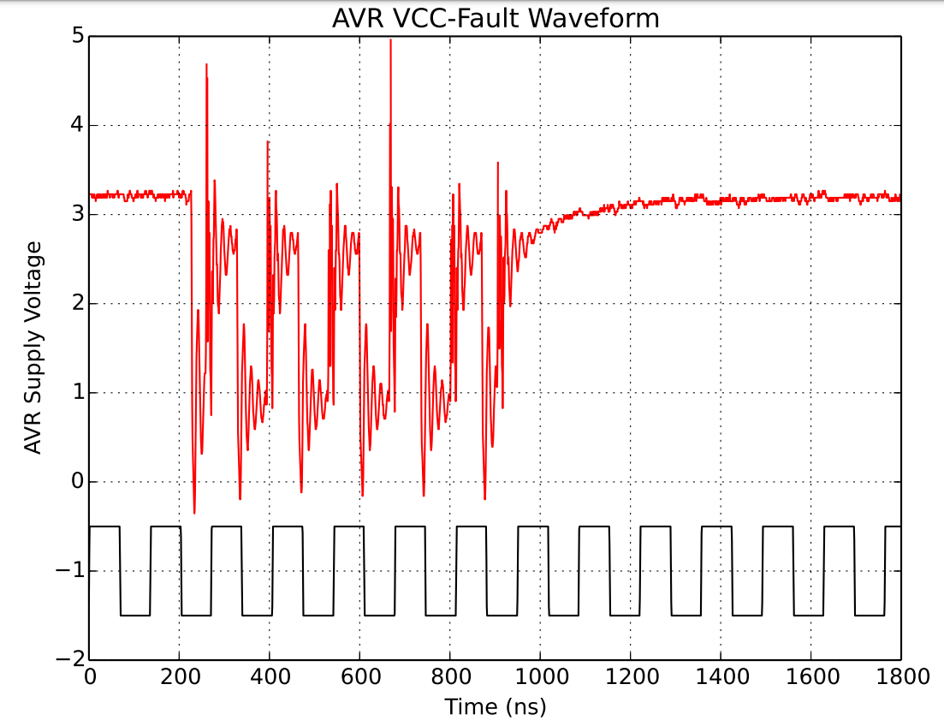
\includegraphics[width=0.5\textwidth]{images/vccSync.png}}
    \caption[Synchronizácia zmeny napätia s hodinami zariadenia.]{Synchronizácia zmeny napätia s hodinami zariadenia. Červenou farbou je znázornená hodnota napätia v čase. V spodnej časti grafu (čierna farba) sú hodinové impulzy zariadenia \cite{crowbars}.}
    \label{obr:vccSync}
\end{figure}

Pre použitie takýchto obvodov je potrebné zabezpečiť, exaktné časovanie generovaných riadiacich impulzov. To je možné zabezpečiť napríklad laboratórnym zdrojom alebo použitím špecializovaného hardvéru, napríklad open source platformu ChipWhisperer \cite{chipwhisperer}. Takéto riešenia však môžu vyžadovať netriviálne náklady. Otázkou je, či aj lacnejšie riešenie, napríklad mikrokontrolér ATMega328P, ktorý je súčasťou populárnych vývojových dosiek Arduino, dokáže dosiahnuť rovnako dobré výsledky. Jedným z cieľov tejto práce je práve vyskúšať takéto typy útokov pomocou mikrokontroléra ATMega328P.

\section{Porucha hodín}
Ďalšou často používanou technikou indukovania chýb je manipulácia taktovacích impulzov prichádzajúcich z externých hodín do zariadenia (angl. clock glitch). Takouto manipuláciou možno vytvoriť nepravidelný taktovací signál, ktorý môže spôsobiť nekorektné správanie hardvéru, ním riadeným. Riadiaca jednotka zariadenia obvykle reaguje na nábehovú (niekedy dobehovú) hranu signálu prichádzajúceho od hodín zariadenia. Napríklad pridanie hrán do takto generovaného signálu môže mať za následok, že sa začne vykonávať ďalšia inštrukcia skôr ako sa predošlá inštrukcia stihla korektne dokončiť, čo pri správnom načasovaní môže spôsobiť cielený efekt na vykonávajúci sa program. Aby bol takýto útok úspešný je potrebné, aby bola riadiaca jednotka zariadenia priamo taktovaná externým oscilátorom. Mnoho zariadení pomocou PLL (Phase Lock Loop) obvodu odvádza z externého signálu od hodín interný, ktorý má rádovo vyššiu frekvenciu. Proti takýmto zariadeniam preto útok touto technikou pravdepodobne nebude účinný\cite{crowbars}.

Útok poruchou hodín môže byť realizovaný napríklad skonštruovaním kombinačného obvodu, ktorý pomocou logických hradiel najčastejšie AND, OR a XOR skladá rôzne výstupné signály zo vstupných. Vstupom do takéhoto obvodu môžu byť rôzne zdroje impulzov napríklad oscilátory s rôznymi frekvenciami, laboratórne zdroje, generátory signálov a ďalšie. Cieľom je rôznymi spôsobmi modulovať výstupný taktovací signál tak, aby v želaných okamihoch mal nesprávny tvar (nepravidelné takty, nesprávne hrany, vyššia frekvencia) a spôsobil tak poruchu na cieľovom zariadení. Pomocou logických hradiel možno vytvoriť rôzne vzorky signálu a následne napríklad využitím multiplexora automatizovane prepínať medzi jednotlivými výstupmi a tým dynamicky meniť výstupný hodinový signál. Na obrázku \ref{obr:clock} je znázornená ukážka schémy takéhoto obvodu \cite{clockCircuit}. Takýto obvod dokonca často nie je potrebné zostaviť fyzicky, ale možno použiť aj programovateľné hradlové pole (FPGA), čo značne zjednoduší implementáciu útoku.

\begin{figure}
    \centerline{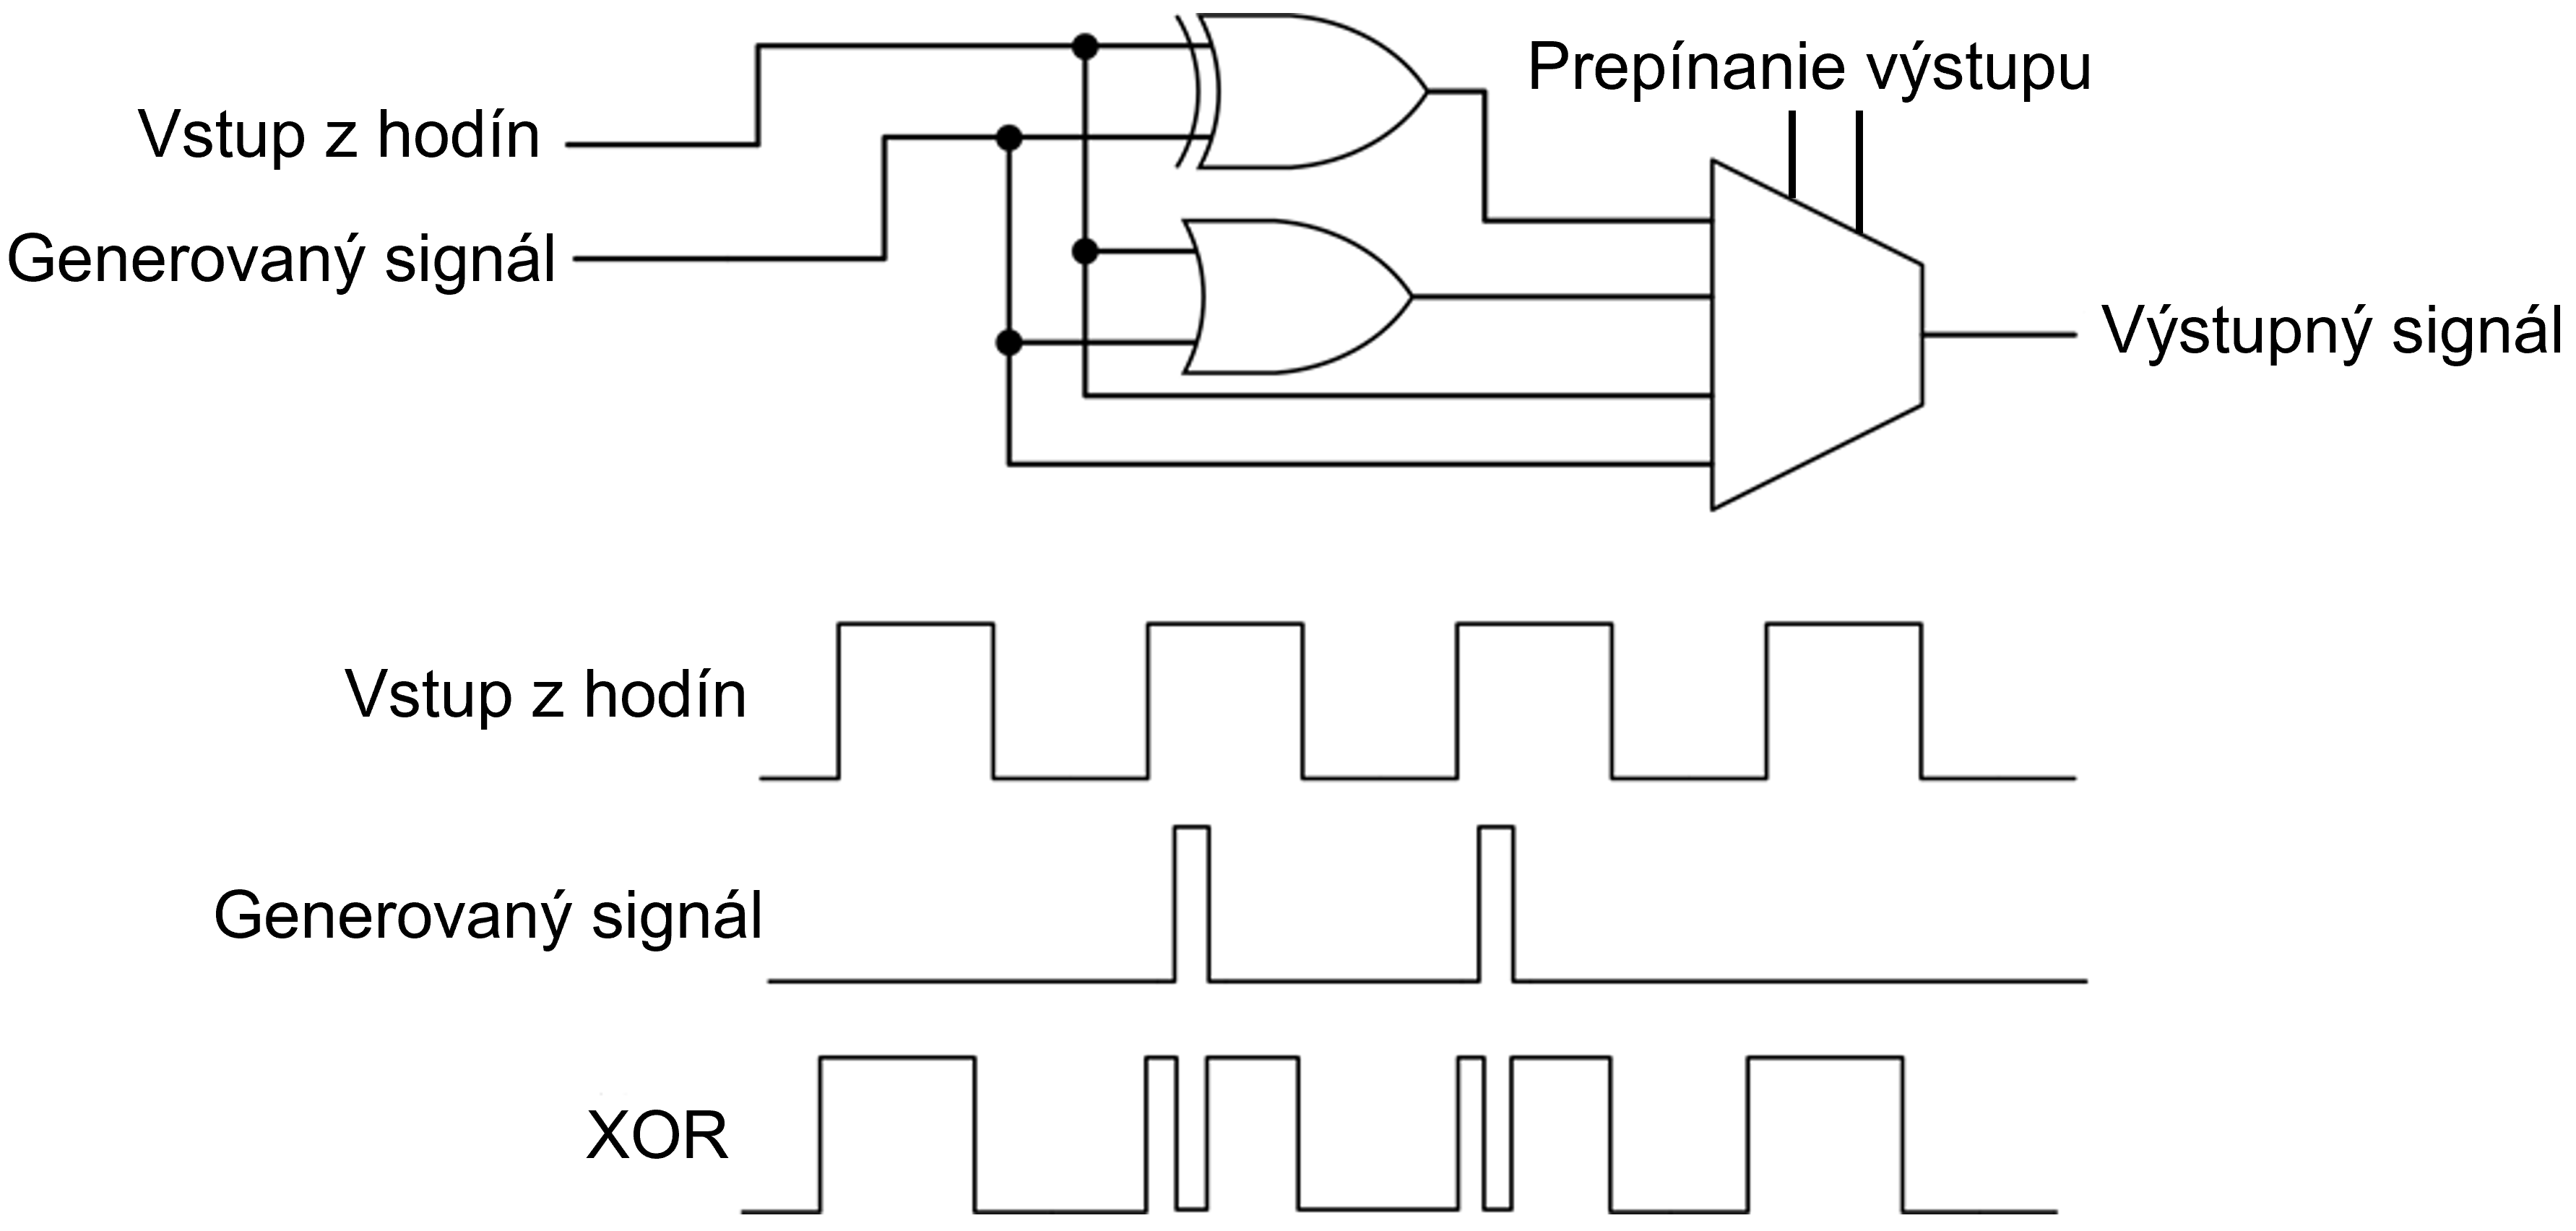
\includegraphics[width=0.75\textwidth]{images/clock.png}}
    \caption[Schéma obvodu pre generovanie nepravidelného signálu.]{Schéma obvodu pre generovanie nepravidelného signálu. Vo vrchnej časti je znázornená schéma obvodu, v spodnej sú rôzne výstupy jednotlivých kanálov multiplexora \cite{clockCircuit}.}
    \label{obr:clock}
\end{figure}

Poruchy, ktoré vieme touto technikou spôsobiť môžu byť rôzne, ale najčastejšie sa týkajú toku riadenia a dát, keďže hodiny generujú signál pre činnosť riadiacej jednotky procesora. Príkladmi takýchto porúch sú vynechanie inštrukcie, nekorektné načítanie dát z pamäte a nekorektný zápis do registra PC (Program Counter), čo môže spôsobiť nesprávny skok vrámci vykonávaného programu. Konkrétna implementácia takéhoto útoku na AVR mikrokontrolér z rodiny ATMega, do ktorej patrí aj nami zvolený ATMega328P (bližšie popísaný v kapitole \ref{kap:hardver}) ukázala, že možno týmto spôsobom vyvolať viaceré z vyššie spomenutých porúch \cite{clock}.

\section{Elektromagnetické rušenie}
Treťou známou technikou indukovania chýb je elektromagnetické rušenie alebo EMFI (Electromagnetic Fault Injection). Vplyvom elektromagnetického poľa možno narúšať fungovanie hardvéru na cieľovom zariadení a tým ovplyvňovať jeho činnosť. Takýto typ útokov zvyčajne vyžaduje XYZ pohyblivú dosku riadenú počítačom, ktorá dokáže hýbať a s dostatočnou presnosťou nastaviť pozíciu antény, ktorá je zdrojom elektromagnetického rušenia. Generátorom impulzov do tejto antény následne možno v daných časových okamihoch spôsobovať želané rušenie \cite{emfi}.

Výhodou tejto techniky je možnosť s istou presnosťou (závisí od parametrov použitej elektroniky) útočiť na konkrétne časti obvodov na cieľovom čipe, napríklad pamäť, registre, či ALU. Nevýhodou je väčšia technická náročnosť útoku a obvykle drahší hardvér.

Existuje mnoho ďalších techník indukovania chýb na hardvéri (napríklad laserové vypaľovanie), ktoré dokážu byť oveľa presnejšie a spoľahlivejšie. Ich implementácia je však prudko náročnejšia, vyžaduje vysokú úroveň technickej odbornosti a veľmi vysoké finančné náklady. Analýza týchto techník preto presahuje rámec tejto práce a nebudeme sa im podrobnejšie venovať.

\section{Ciele útokov}
Najčastejším cieľom útokov pomocou indukovania chýb je obídenie bezpečnostného mechanizmu. Jednoduchým príkladom je ovplyvnenie jednoduchej kontroly podmienky v programe vyvolaním chyby, ktorá spôsobí skočenie programu do nesprávnej vetvy, čo z vyššieho pohľadu môže mať efekt nesprávneho vyhodnotenia tejto podmienky. Zložitejšie útoky môžu cieliť na nesprávne vykonanie aritmetickej, či logickej operácie alebo nekorektné prečítanie dát z pamäte a následne chybné rozhodnutie algoritmu, čo spôsobí cielené obídenie daného bezpečnostného mechanizmu. Konkrétnym príkladom takýchto cieľov môže byť získanie neoprávneného prístupu k službám alebo dátam zariadenia, prečítanie obsahu pamäte s firmvérom aj pri zapnutej ochrane pred čítaním, útok na zavádzací softvér počítača, aby naštartoval systém z nepovoleného média a množstvo ďalších scenárov.

Ďalšia kategória cieľov týchto útokov sú zariadenia implementujúce kryptografické schémy. Tieto schémy sú často veľmi náchylné na implementačné chyby a preto dopady takýchto útokov môžu byť fatálne. Pomocou indukovania chýb možno napríklad prinútiť zariadenie, aby použilo nulový vektor ako kľúč pre symetrickú šifru. Potom už je jednoduché takto zašifrované dáta priamo dešifrovať. O niečo sofistikovanejšia, ale o to účinnejšia, metóda útokov na kryptografické konštrukcie je tzv. DFA (Differential Fault Analysis). Princíp tejto metódy spočíva v indukovaní chýb na kryptografický algoritmus a porovnávaním korektných a nekorektných výstupov určiť aké inštrukcie a dáta sa v zariadení spracovávaj. Takouto analýzou je následne možné napríklad určiť použitý kľúč v symetrickej šifre alebo dokonca efektívne faktorizovať verejný modulus RSA schémy. Praktická úspešnosť týchto útokov bola demonštrovaná proti implementáciám schém AES a RSA na vnorených zariadeniach \cite{crypto}.

\section{Zraniteľnosti a obranné mechanizmy}
Samotná implementácia a následná úspešnosť útoku často závisí aj od samotného algoritmu, na ktorý je útok cielený, a spôsobu jeho implementácie. Rôzny kód môže mať rôzne druhy zraniteľností a od toho sa odvíja ako veľmi môže byť náročná technická realizácia útoku. Niekedy nie je pre dosiahnutie cieleného efektu potrebné mieriť na jednú konkrétnu chúlostivú operáciu, ale stačí pokiaľ je výsledok série operácií nesprávny. Príkladom kódu, ktorý je náchylný voči chybám spôsobeným vplyvom prostredia je postupné inkrementovanie premennej v rámci cyklu, alebo séria viacerých priradení do rovnakej premennej počas výpočtu. Kedy presne nastane chyba neovplyvní výsledný efekt útoku, za predpokladu, že chyba nespôsobí fatálne zlyhanie cieľového zariadenia. Pre tento typ útokov je často postačujúci lacný hardvér a nie je väčšinou potrebná synchronizácia zdroja chýb a cieľa.

V iných prípadoch je potrebné cieliť na konkrétnu operáciu, čo zvyčajne vyžaduje vyššiu presnosť a synchronizáciu zariadení počas útoku. Príkladom takejto zraniteľnosti je zneužitie jednoduchej optimalizácie kompilátora \cite{AntiFI}. Kompilátor pri prekladaní cyklu, v ktorom sa postupne dekrementovala iterovaná premenná a postupne čítal vybraný úsek pamäte, použil inštrukciu BNE (Branch if Not Equal) miesto BLT (Branch if Less Than). Takáto optimalizácia je z teoretického pohľadu správna, keďže nemení význam algoritmu a test na nulu možno efektívnejšie vykonať ako všeobecné porovnanie. Keď v takto upravenom programe docielime vynechanie tejto inštrukcie práve vtedy, keď má dôjsť k ukončeniu cyklu, spôsobíme tým, že  takýto program bude pokračovať v cykle až kým nepretečie hodnota iterovanej premennej. Takýto útok bol demonštrovaný a autorovi sa podarilo prečítať firmvér na mikrokontroléri napriek tomu, že k nemu nemal oprávnený prístup. V prípade, že by kompilátor použil inštrukciu BLT, by bolo potrebné pravidelne v každej iterácií spôsobiť takúto chybu, čo je pre útočníka náročnejšie \cite{AntiFI}.

Existuje viacero obranných mechanizmov, ktoré dokážu takéto útoky skomplikovať, niekedy až znemožniť. Medzi aktívne mechanizmy patrí detekcia takýchto útokov s využitím špecializovaného hardvéru, alebo softvéru a následne spustiť bezpečnostné opatrenie, napríklad reštart zariadenia. Aktívna detekcia útokov zvyšuje výkon zariadenia, čo najmä v prípade vnorených systémov môže byť problematické riešenie. Jednoduchší, ale niekedy postačujúci, je pasívny spôsob obrany, napíklad úprava kódu tak, aby bol menej chúlostivý voči chybám. Pridanie náhodných oneskorení do programu môže sťažiť situáciu útočníkovi, ktorý potrebuje presne načasovať útok na konkrétnu operáciu. Ďalšími opatreniami môže byť nepoužívanie binárnych premenných pri vetvení programu a rovnako nepoužívanie triviálnych konštánt (0, súvislý vektor jednotiek). Nastavenie konkrétnej netriviálnej hodnoty (0xAA, 0xB9, ...) vplyvom chyby je náročnejšie, niekedy zanedbateľne nepravdepodobné a možno tak takémuto útoku zabrániť.